\documentclass[,a4paper,12pt,french]{article}

\usepackage[TD]{../../../Style}

\pagestyle{empty}

% Début du document
%%%%%%%%%%%%%%%%%%%
\begin{document}

\titre{Fonctions affines - Exercices}

\begin{multicols*}{2}
\begin{exercice}
Parmi les fonctions suivantes, lesquelles sont des fonctions affines? Identifier $a$ et $b$ dès que possible.

\begin{centrer}
$ f:x \mapsto 3x-2 \hfill g:x \mapsto x^2 \hfill h:x \mapsto 1$

$\hfill i:x \mapsto \frac 1 x + 1 \hfill$
\end{centrer}
\end{exercice}

\begin{exercice} \label{exorep} \ 

Associer aux trois droites ci-dessous la fonction affine qui leur est associée parmi les suivantes:

\begin{centrer}
$f:x \mapsto 2x \ , \ g:x \mapsto -0.5x+2 \ , \ h:x \mapsto \frac x 5 +1$
\end{centrer}

\begin{centrer}
\begin{tikzpicture}[scale=\echellepgf]
\begin{axis}[
styleglobal,
width=0.95*\echellepgfinv*\linewidth,
xmin=-3, xmax=9,
ymin=-2, ymax=4,
xtick distance=1,
ytick distance=1,
]
\addplot[styleplot,domain=(-9:9)]{2*x};
\addplot[color=red,styleplot,densely dashed,domain=(-9:9)]{-0.5*x+2};
\addplot[color=blue,styleplot,densely dotted,domain=(-9:9)]{0.2*x+1};
\end{axis}
\end{tikzpicture}
\end{centrer}

\end{exercice}

\begin{exercice}
Représenter sur un même repère les droites d'équation $y=3x-1$ et $y=3-\frac 1 3 x$, puis déterminer graphiquement les coordonnées de leur point d'intersection.

\begin{centrer}
\begin{tikzpicture}[scale=\echellepgf]
\begin{axis}[
styleglobal,
width=0.95*\echellepgfinv*\linewidth,
xmin=-3, xmax=9,
ymin=-2, ymax=4,
xtick distance=1,
ytick distance=1,
]
\end{axis}
\end{tikzpicture}
\end{centrer}
\end{exercice}

\begin{exercice}
Représenter sur un même repère les droites suivantes:
\begin{itemize}
\item $d_1$ passant par $A(0;-1)$ et de coefficient directeur $1$
\item $d_2$ passant par $B(-3;2)$ et de coefficient directeur $-2$
\item $d_3$ passant par $C(-1;1)$ et de coefficient directeur $\frac 1 2$
\end{itemize}
\end{exercice}

\begin{exercice}
Trouver l'équation réduite de chaque droite:

\begin{centrer}
\begin{tikzpicture}[scale=\echellepgf]
\begin{axis}[
styleglobal,
width=0.95*\echellepgfinv*\linewidth,
xmin=-3, xmax=9,
ymin=-2, ymax=4,
xtick distance=1,
ytick distance=1,
%major grid style={line width=1pt},
]
\addplot[styleplot,domain=(-1:3)]{3*x-0.5} node[pos=0.55,right] {$d_1$};
\addplot[color=red,styleplot,densely dashed,domain=(-9:9)]{0.25*x+2} node[pos=0.9,below] {$d_2$};
\addplot[color=blue,styleplot,densely dotted,domain=(-9:9)]{-0.5*x+1} node[pos=0.8,above right] {$d_3$};
\end{axis}
\end{tikzpicture}
\end{centrer}
\end{exercice}

\begin{exercice}
Par lecture graphique, retrouver les équations des trois droites de l'exercice \ref{exorep}.
\end{exercice}

\begin{exercice}
Déterminer l'équation réduite des droites suivantes:
\begin{itemize}
\item $d_1$ qui passe par $A_1(0;1)$ et $B_1(2;5)$
\item $d_2$ qui passe par $A_2(-3;5)$ et $B_2(1;-7)$
\item $d_3$ qui passe par $A_3(2;0.5)$ et $B_3(-1;-1)$
\end{itemize}
\end{exercice}

\begin{exercice}
Dresser le tableau de signes des fonctions affines suivantes:

\begin{centrer}
$f:x \mapsto 3x-2 \hfill g:x \mapsto 2-5x \hfill h:x \mapsto \frac 1 2 + 4x$

$\hfill i:x \mapsto -(x-4)+3x-1 \hfill j:x \mapsto \frac x 4 - \frac 2 3 \hfill$
\end{centrer}
\end{exercice}

\begin{exercice}
Dresser le tableau de signes de \\ $f:x \mapsto (x-1)(2+x)$:

\begin{center}
\begin{tikzpicture}
\tkzTabInit[lgt=1.2]{$x$ /1, $x-1$/1, $2+x$/1,$f(x)$/1}{,,}
\end{tikzpicture}
\end{center}
\end{exercice}

\begin{exercice}
Dresser le tableau de signes des fonctions:
\begin{itemize}
\item $f:x \mapsto 3(2x-4)(3x+6)$
\item $g:x \mapsto -2(3x-5)(4-8x)$
\end{itemize}
\end{exercice}

\end{multicols*}

\end{document}
